\newpage
\section{Satellite Galaxy Haloes}

In this problem, we create a number density profile for satellites galaxies in a dark matter halo. The profile is defined as
\begin{equation}
    n ( x ) = A \left\langle N _ { \mathrm { sat } } \right\rangle \left( \frac { x } { b } \right) ^ { a - 3 } \exp \left[ - \left( \frac { x } { b } \right) ^ { c } \right]
    \label{eq:n(x)}
\end{equation}

I created class called \texttt{GalaxyProfile} for easy usage of this profile:

\lstinputlisting[language=Python, caption=\texttt{gal\_profile.py}]{nur/gal_profile.py}

The integration and derivation routines can be found in Appendices \ref{sec:integration} and \ref{sec:derivation} respectively. More detail is also given in the following sections.


    \newpage
    \subsection{Random values for a, b, and c}

    When calling \texttt{GalaxyProfile} without specifying the free parameters $a$, $b$, and $c$, the class automatically generates random numbers for these in the range specified by the assignment sheet. 

    The class then finds the normalization factor $A$ using a spherical integrator, which in turn uses Simpson integration. While I did also implement a trapezoidal integrator (see Appendix \ref{sec:integration}), timing tests showed that Simpson was slightly faster for spherical integration.

    \lstinputlisting[language=Python, caption={\texttt{integration.py} : simpson, spherical}, firstline=19, lastline=48]{nur/integration.py}


    Printing the object then shows the values for the generated parameters:

    \lstinputlisting[language=Python, caption=\texttt{handin1.py} : 2a,
                     firstline=74, lastline=77]{handin1.py}
    \lstinputlisting{output/2a.txt}

    

    \newpage
    \subsection{Interpolation}

    I used two different interpolators -- linear and polynomial via Neville's algorithm -- to attempt this problem. The full code (including the \texttt{bisect()} function used by \texttt{linear()}) is available in Appendix \ref{sec:interpolation}.

    \lstinputlisting[language=Python, caption=\texttt{interpolation.py} : linear, firstline=40, lastline=78]{nur/interpolation.py}

    \lstinputlisting[language=Python, caption=\texttt{interpolation.py} : polynomial, firstline=81, lastline=114]{nur/interpolation.py}

    \lstinputlisting[language=Python, caption=\texttt{handin1.py} : 2b,
                     firstline=89, lastline=123]{handin1.py}

    \begin{figure}[H]
        \centering
        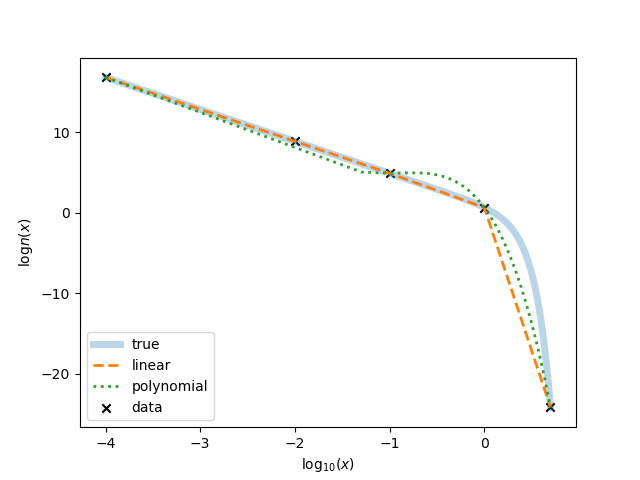
\includegraphics[width=.5\textwidth]{output/2b_interpolation.png}
        \caption{Interpolation between data points using two different interpolation schemes.}
    \end{figure}

    Both methods seem roughly comparable for the 100 interpolated points, however as \texttt{len(xinterp)} increases, \texttt{polynomial()} performs worse. I interpret this to mean that the fewer the points, the more \texttt{polynomial()} approximates \texttt{linear()} and performs better. This means that \texttt{linear} is the more appropriate interpolator for this problem.



    \newpage
    \subsection{Derivation}

    I used the central difference formula to find the derivative of Equation \ref{eq:n(x)} at the generated value for $b$. 

    This was implemented as a method \texttt{dn()} for the \texttt{GalaxyProfile} class.

    \lstinputlisting[language=Python, caption=\texttt{derivation.py} : central, firstline=6, lastline=12]{nur/derivation.py}
    
    \lstinputlisting[language=Python, caption=\texttt{handin1.py} : 2c,
                     firstline=133, lastline=133]{handin1.py}

    \lstinputlisting{output/2c_derivative.txt}

    I did not get a chance to calculate the error or compare the numerical derivation to the analytical value.



    \newpage
    \subsection{Galaxy position generation in 3D}

    There are two parts to this problem: First for sampling the radius and second for the angles.

    I sample the probability distribution, 
    \begin{equation}
        P(x) dx  = n(x) \cdot 4 \pi x^2 dx / \langle N_{sat} \rangle
        \label{eq:p(x)}
    \end{equation}

    using rejection sampling. Although this method is often slow, I found that this function was broad enough that the number of attempts to sample from the distribution was still reasonable. 


    \lstinputlisting[language=Python, caption=\texttt{sampling.py} : rejection, firstline=8, lastline=39]{nur/sampling.py}


    \newpage
    The next step is to sample $\theta$ and $\phi$ from a spherical distribution. 

    \lstinputlisting[language=Python, caption=\texttt{sampling.py} : spherical, firstline=42, lastline=54]{nur/sampling.py}

    
    With these two sampling functions defined, a set a box around the function and sample from within the box to find $x$. For each $x$ value found, I then randomly generate values for $\theta$ and $\phi$.
    
    \lstinputlisting[language=Python, caption=\texttt{handin1.py} : 2d,
                     firstline=149, lastline=171]{handin1.py}

    \begin{figure}[H]
        \centering
        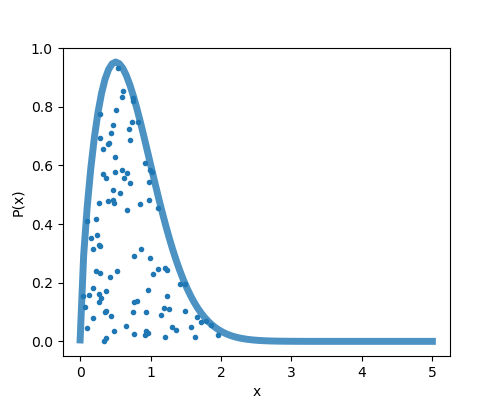
\includegraphics[width=.5\textwidth]{output/2d_r-samples.png}
        \caption{Sampling P(x) with rejection sampling}
    \end{figure}


    Below is the first ten of the 100 galaxies generated. The full list can be seen in Appendix \ref{sec:gal_gen}

    \lstinputlisting[caption=\texttt{galaxies.csv}, firstline=1, lastline=11]{output/2d_galaxies.csv}


    \newpage
    \subsection{1000 haloes}

    Here, I create 1000 haloes with 100 satellites each, drawing $x$ from the distribution:

    \begin{equation}
        N(x) = n(x) \cdot 4 \pi x^2
    \end{equation}

    I save these values in a (1000x3x100) datacube, which I then use to average all 1000 haloes in $x$ to create a histogram.

    \lstinputlisting[language=Python, caption=\texttt{handin1.py} : 2e,
                     firstline=184, lastline=220]{handin1.py}

    \begin{figure}[H]
        \centering
        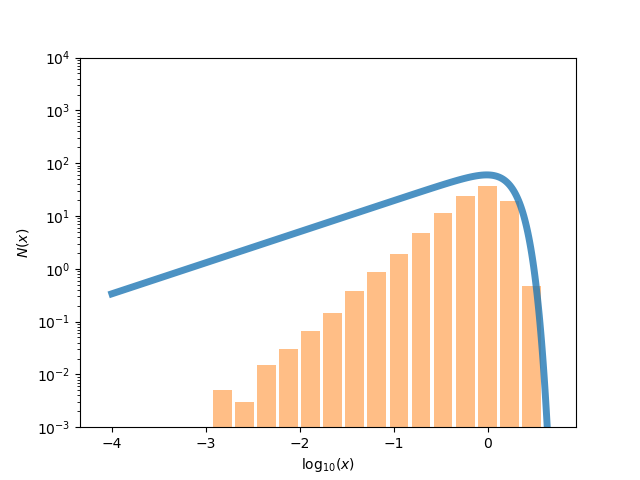
\includegraphics[width=.5\textwidth]{output/2e_average-r.png}
        \caption{Average values of $x$ for 1000 haloes compared to $N(x)$}
    \end{figure}



    \newpage
    \subsection{Minimization and root finding}

    In order to find the solutions of $N(x) = N_{max}/2$, I first found the function maximum using a golden ratio search. This method quickly converges if the initial bracket is small, however it is difficult to generalize for this problem as if the bracket is too large it is very slow to converge (and often does not find the maximum at all).

    \lstinputlisting[language=Python, caption=\texttt{minimization.py}]{nur/minimization.py}

    Next, I shift the function down by $N_{max}/2$ in order to use root-finding to find the $x$-values. The algorithm I use is bisection, which iteratively checks if the root is between two points and then tightens the bracket.

    \lstinputlisting[language=Python, caption=\texttt{root\_finding.py}]{nur/root_finding.py}


    \lstinputlisting[language=Python, caption=\texttt{handin1.py} : 2f,
                     firstline=230, lastline=267]{handin1.py}

    \begin{figure}[H]
        \centering
        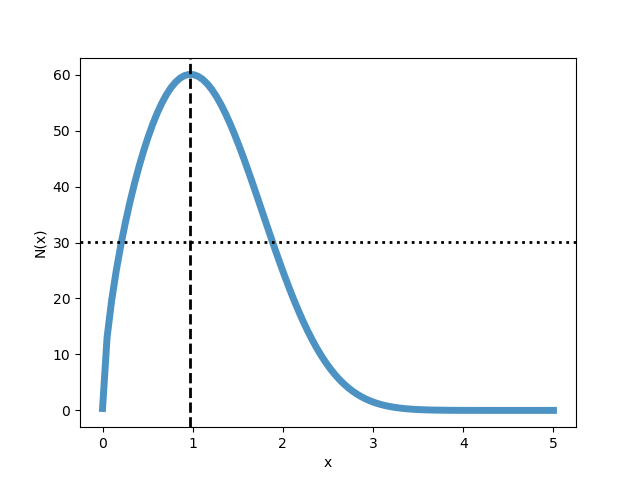
\includegraphics[width=.45\textwidth]{output/2f_max.png}
        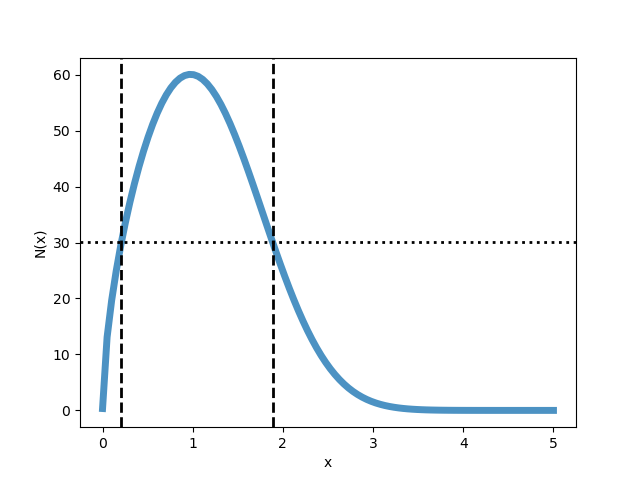
\includegraphics[width=.45\textwidth]{output/2f_roots.png}
        \caption{The location of the maximum and $N_{max}/2$ (left) and the solutions to the roots (right).}
    \end{figure}

    \lstinputlisting[caption=\texttt{2f\_roots.txt}]{output/2f_roots.txt}


    \newpage
    \subsection{Sorting and comparison with Poisson distribution}

    In order to sort the values in the largest bin, I first attempted to do a heap sort. I was able to successfully put a list of around 10 values into a heap, however once I tried it with the 1000 values it failed to sort it correctly. My attempt can be seen in Appendix \ref{sec:sorting}. 

    Failing the heap sort, I opted to use quick sort instead, which recursively choices a pivot point and sorts the values to the left and then to the right.

    Once the values are sorted, I find the median, the 16th and 84th percentiles, and finally I put the galaxies in the max radial bin into a histogram and compare it to the Poisson distribution.

    \lstinputlisting[language=Python, caption=\texttt{sorting.py} : quick sort,
                     firstline=6, lastline=34]{nur/sorting.py}


    \lstinputlisting[language=Python, caption=\texttt{handin1.py} : 2g,
                     firstline=281, lastline=313]{handin1.py}

    \lstinputlisting{output/2g_median-percentiles.txt}

    \begin{figure}[H]
        \centering
        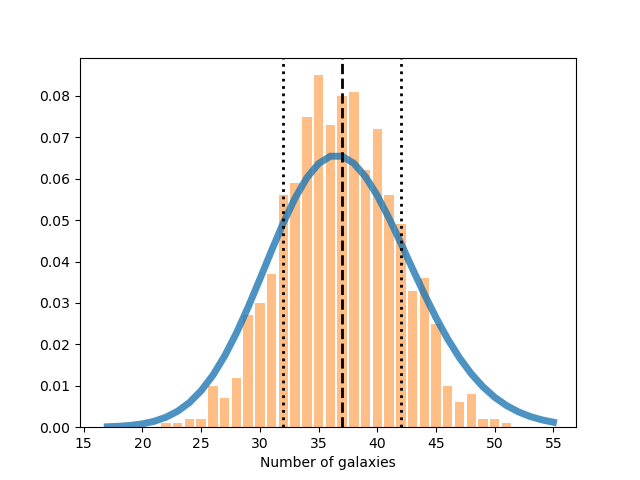
\includegraphics[width=.5\textwidth]{output/2g_ngal.png}
        \caption{The number of galaxies in the maximum radial bin for 1000 haloes as compared to the Poisson distribution. The vertical lines show the median and 16th and 84th percentiles. As can be seen, the distribution of galaxies follows the Poisson distribution quite well.}
    \end{figure}



    \newpage
    \subsection{Finding A}

    I was able to find all 6240 values of A however I was not able to write the 3D interpolator. This method ended up being quite slow -- it takes around 1.2 seconds to find A for a single realization of a, b, and c, but with 6240 values this ended up taking 2 hours to run. I saved the output in a file which then can be loaded for future use.

    \lstinputlisting[language=Python, caption=\texttt{handin1.py} : 2f,
                     firstline=325, lastline=353]{handin1.py}
